\section{Checkpoint}
Akhila, Amin, and Amit were responsible for the checkpoint submodule, and with the help of Amin, most of the part was reformatted, debugged, and security fixes were made. In this section, we discuss how participants receive a stable state in the network through the checkpoint. Also, the functioning of the checkpoint module is divided into two modules. One handles checkpoint calculation and verification, and the second handles consensus and exchange of checkpoint with the network.
\subsection{Introduction to Checkpoint}
%solid

Distributed systems rely on the shared state of the network to store and process the transaction ledger. Ledger size starting from genesis to present transaction can become too large and grow over time, making the system less efficient by updating new participants. It is also a hurdle to process old transactions and create unnecessary network traffic to get an inefficient update. By generating Checkpoints, we allow new participants to grasp the latest network state and old participants to remove redundant data. The system does not require old transactions to be stored that were resolved by checkpoint generation, the agent can store them, but the system does not need it to run. In short, the checkpoint becomes a new genesis for all participants, which includes the set of unspent transaction outputs since the last checkpoint, stake ownership, and total stake in the system. 

\subsection{Terms and Assumptions}
\textbf{Terms}
\begin{itemize}
\item A participant in the system is called an agent, and if an agent owns some stake in the system and issues acknowledgment, then we consider it a validator.
\item The term Fee and Rewards can be used interchangeably. Comparatively to other transaction systems, ABC uses a special incentive mechanism where incentives are correlated to the fees earned and awarded with the fees.
\end{itemize}
\textbf{Assumption}
\begin{itemize}
\item We assume that the validators members keep a record of the full DAG since the last checkpoint as it is needed to resolve upcoming transactions and create a new checkpoint.
\item The total amount of money in the system is always equal to the total amount of the system's stake. 

\end{itemize}

\subsection{Working}
%Trigger
%dag traversal
%calculation
The checkpoint is triggered after every constant amount of time, and there is no need to have a global time in the network as the proposed checkpoint can be voted down by other agents if it happens too frequently. This gives the majority of stake holder an upper hand to decide on the decision.  
Delaying checkpoint creation will not reward validators any further, but it will also delay future checkpoints where the validator might benefit from again. So, it's in the interest of the stakeholders to release checkpoints regularly.
Besides, checkpoints must have at least one transaction, or else the system ignores the empty checkpoint immediately. The major leap in checkpoint creation is that it can be mapped to a particular transaction due to the output wallets' uniqueness. The checkpoint validation also relies on the transaction validation process to resolve transaction conflicts and double-spending. No unconfirmed transaction can end up in the checkpoint because most participants will only have confirmed transactions in their DAG. The Figure \ref{{fig:ckpt_transition} summarizes the process of checkpoint transition. It is interesting to note that the conflict does not arise even if the wallets which checkpoint summarizes have to be spent by another transaction as the validation of checkpoint relies on unique wallets. If a valid transaction is found for the spent wallet, this wallet will be removed from the local state and summarized in the next checkpoint. 
\begin{figure}
    \centering
    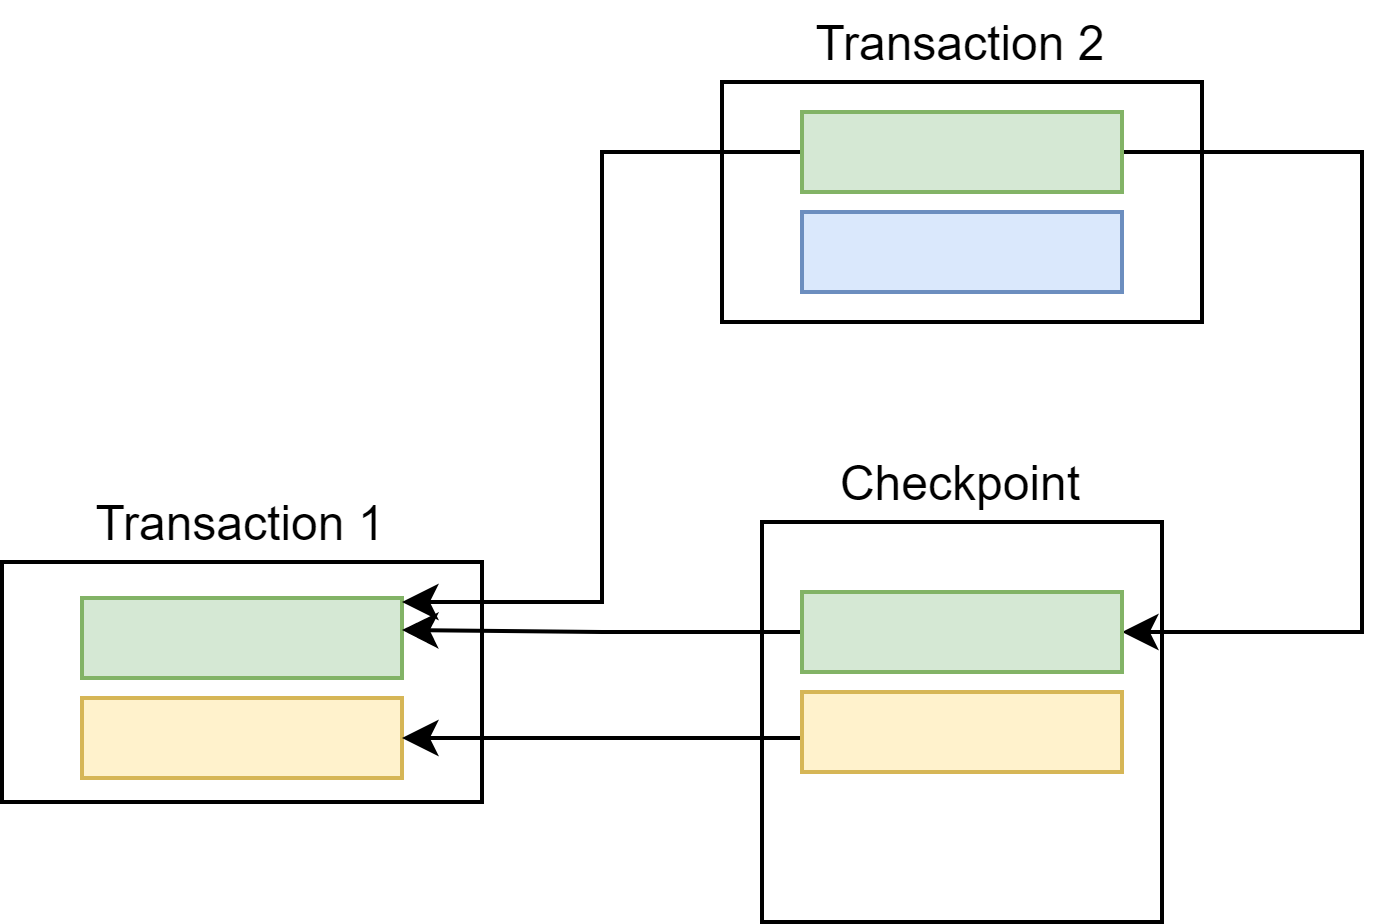
\includegraphics[width=100mm,scale=0.4]{figures/drawio/transition.png}
    \caption{Resolving transaction link during transition}
    \label{fig:ckpt_transition}
\end{figure}
%dag traversal
The agent calculates the checkpoint data concerning it is local DAG only when the trigger initiates it. There is no calculation after confirmation of each transaction or after receiving an acknowledgment. The checkpoint summarizes all the unspent outputs extracted from the transaction according to its local DAG structure and rewards the fee to acknowledgments made. The fee calculation, and generation of new money by incentives are discussed in Incentives chapter.

The calculation of checkpoint is dependent on unique identifiers of the wallets and transaction identifiers. Unique identifier of the wallets helps the system to track ownership of the wallets while transaction in the ABC summarizes the generation of these wallets and validator identification. 
\begin{figure}
    \centering
    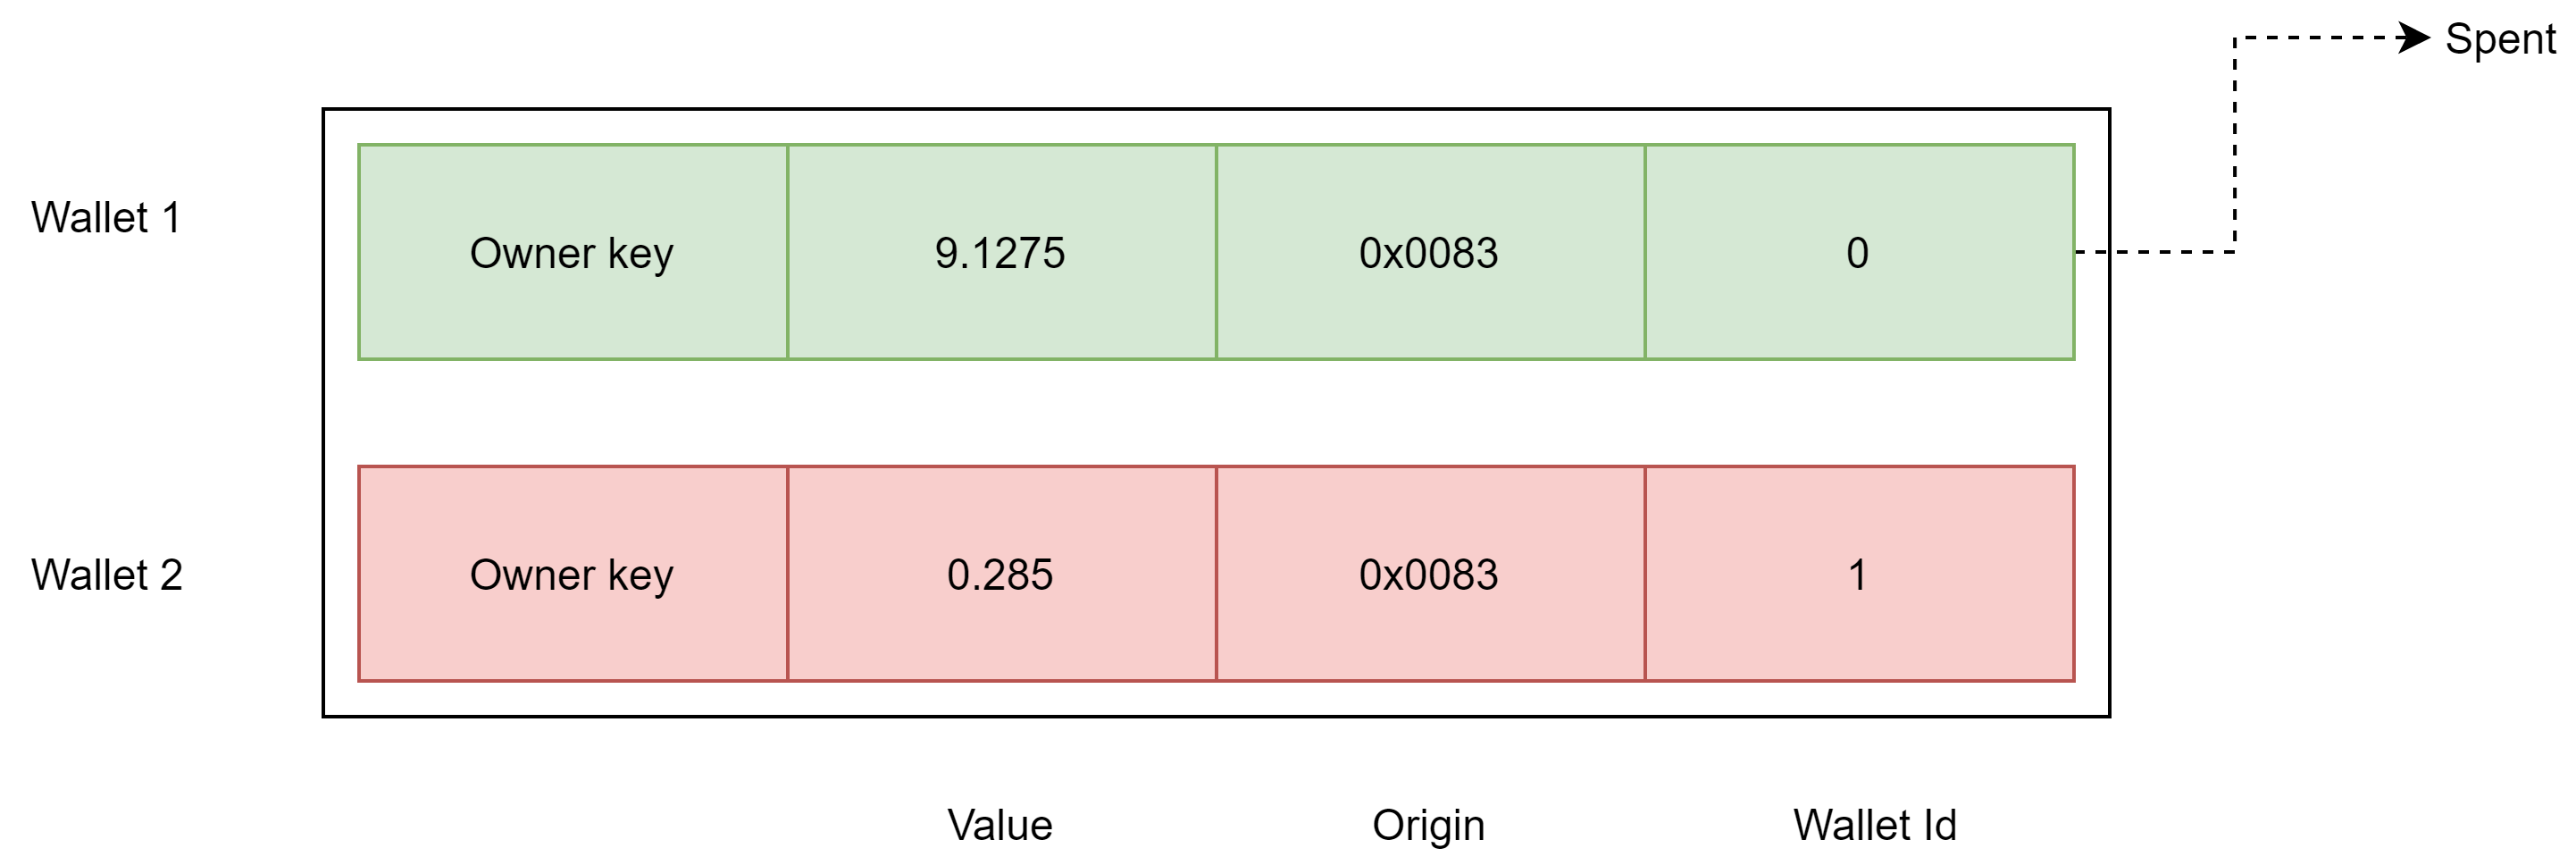
\includegraphics[width=125mm,scale=0.5]{figures/drawio/wallet_demo (1).png}
    \caption{Output list of a transaction}
    \label{fig:ckpt_wallet}
\end{figure}
The Figure \ref{fig:ckpt_wallet} represents a list of output wallets in a transaction where each wallet can be identified by its origin combined with its id. The checkpoint calculation considers transactions as the only basis of stake calculation and wallets for ownership. The wallets can only be used in a transaction by their owners. The summarized list of the checkpoint output is always considered unspent, if no transaction can be found for the respective wallets in the future. 
\subsection{Incentives}\label{incentive}
%fee calculation
Fees and incentives are some of the lucrative attributes for validators, directly related to honest behavior in the system. The mechanism also encourages participants to partake in the system actively. It is not unusual to charge fees for transactions in any transaction system, however ABC is different. The fees are given to the validator who acknowledges the transaction, and if all validators with a combined stake of  2/3 of the total stake acknowledge it, it is considered confirmed. The ABC's specialty is that the validator also receives an incentive on top of the original fee amount. The incetive is generated as new money to counter inflanation and to cover the loss of money if some validators did not acknowledge the transaction.
The incentive is calculated with the following equation:

\begin{equation}
\alpha\dfrac{m}{M}fee(x)
\end{equation}

Here, constant alpha is a constant factor that decides incentive percentage, $m$ is the validator's stake, and $M$ is the total stake present in the system. The transaction will incur fees as long as the m is less than 1/3 of the total stake, and alpha constant in the range: $$1<\alpha<3$$
%money generation example
Let us assume that a transaction txn with fee amount 10 is issued by an agent that holds stake 100(m) and total stake in the system where $$\alpha=1.5$$ is 1000(M). As the same agent holds the stake, it can acknowledge for its transaction and receive incentive. In this case, the incentive for the agent is:
$$1.5 = 1.5 \times \dfrac{10}{100} \times 10$$ In this manner, if all other agents are having a stake in the system issue an acknowledgment, will receive the amount, and the money generated for the number of fees 10 units will be 5 units. If some of the agents who hold stake(<1/3) in the system do not acknowledge the transaction, and the transaction is confirmed, the amount generated will be less, but no money will be lost.
$$1.5 \times \dfrac{2}{3} \times 10 = 10$$ which is the exact amount of money taken as fees.
In another scenario, where $$\alpha>3$$ and the issuer's stake is more than or equal to 1/3 in the system, the issuer will pay fees but earns it back by acknowledging the same transaction.
$$3 \times \dfrac{1}{3} \times 10 = fee$$ for the transaction. The adversary can misuse this scenario to attack the system by injecting more transactions into the system as it pays no fees for the same. The issue can be solved by using $$\alpha<3$$ According to our assumption, more than 2/3 of the stake should be held by honest agents, which reassures the system functionality. The checkpoint submodule calculates final fees for all the validators w.r.t acknowledgments present in the DAG and concludes the fee distribution to the checkpoint. The stake for the fee amount goes to its owners. The fees are included in the checkpoint as a separate wallet list, and the origin of these wallet is set to the checkpoint's identifier as the new money has no origin. Once a checkpoint is confirmed, the fees earned can be spent as regular money. The checkpoint also summarizes the total stake owned by a validator as a list similar to unspent outputs and reward wallets. The total amount of the stake is equal to the real money in the system, and the stake is correlated to money owned, but changed by the validator attribute in a transaction. Each transaction issuer has a right to delegate the stake to any validator it chooses. Also, with the same property, the receiver can change the validator of its choosing, but it incurs a charge. To switch to a validator of its choosing, one needs to initiate a transaction where the sender will be the receiver. Still, the validator tag of the transaction will have an expected identifier change. The ABC's stake property is fascinating, and there's more on which the system can rely to limit adversarial behavior and incentivize participants. The author of ABC \cite{abc_paper}  suggested many ideas which reimburse transaction issuers for delegating the stake. In this manner, the transaction issuer will also become a part of the system compared to other existing systems where the issuer is only using the service. These missing parts can be explored and researched. 
%money destruction
Each checkpoint also generates a certain amount of new money by rewarding the consensus protocol winner, proposing the checkpoint.  
Checkpoint proposer will be automatically awarded for the creation of a checkpoint once confirmed. The amount can be agreed upon by the validator after respective time with a consensus mechanism or remain constant as acknowledgment is the primary source of money generation.  One note here would be that the amount of money generated in each checkpoint relates to the transactions confirmed since the last checkpoint.
\subsection{Validation}
% checkpoint chain
The checkpoint validation happens in the same manner as it is generated. Each participant who votes for the checkpoint verifies the wallets summarized inside the checkpoint respective to its DAG and validates it. There might be a case where some transactions are found missing, and these transactions can be requested from the network and then validated. If there exists no such transaction, the validator does not vote for the checkpoint. Each checkpoint contains an identifier of the last checkpoint, which can not be altered. With validation in mind, the participant also validates the checkpoint by analyzing the checkpoint chain mapping back to genesis. All the participants repeat this process. It is possible because the active validators in the system store all the checkpoints since genesis. This mechanism can be simplified in future work, but it is effective validation for new participants, since they might not have the history. 
\begin{figure}
    \centering
    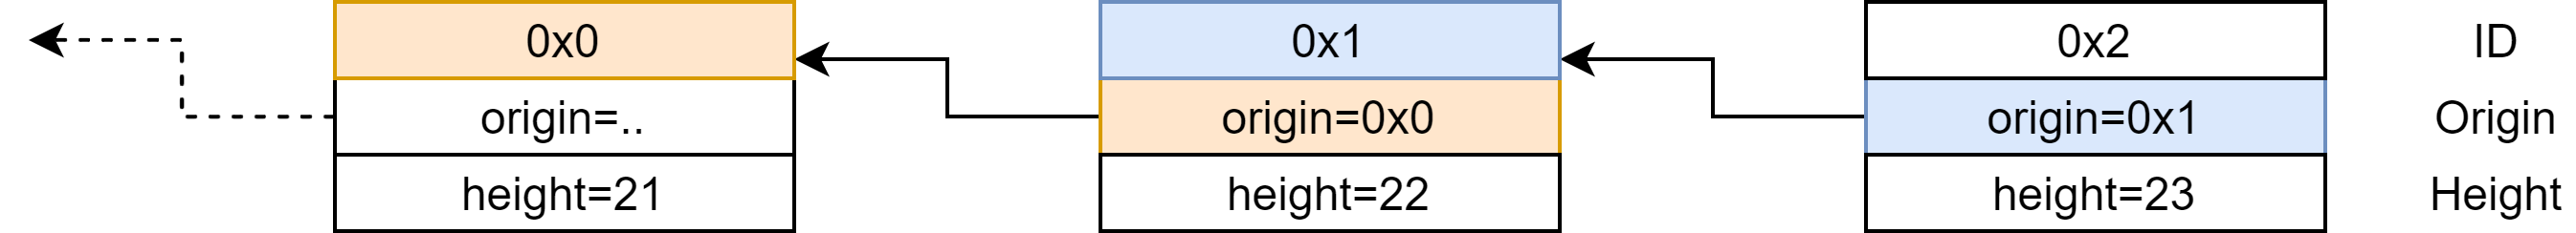
\includegraphics[width=125mm,scale=0.5]{figures/drawio/checkpoint_demo.png}
    \caption{Checkpoint chain}
    \label{fig:ckpt_demo}
\end{figure}
The Figure \ref{fig:ckpt_demo} explains the checkpoint chain mapping with the help of origin. One point to note here would be to consider the height and identifier, as the identifier does not explain the checkpoint number. The validation process also validates the height of the checkpoint.
\subsection{Design of Checkpoint Service}
The checkpoint service module \ref{fig:ckptservice_dependency} performs all the calculations and validation related to checkpoints in the project. The checkpoint service module is relatively small compared to other module implementation, but efficient in processing the checkpoint and storing them in a database. The checkpoint service is injected into the abccore, module as dependency injection and inherits data structures from abccore to process the DAG, including transactions, acknowledgments, and checkpoints. The Consensus mechanism also uses the checkpoint service to exchange checkpoints from other participants and provides the validation status back to the consensus. The checkpoint's main structure resides in the abccore as it provides all the basic structures to other modules. 
\begin{figure}
    \centering
    \includegraphics[width=125mm,scale=0.5]{figures/drawio/dependency_ckptservice1.pdf}
    \caption{Checkpoint Service dependency diagram}
    \label{fig:ckptservice_dependency}
\end{figure}
